\chapter{State of the art} % Main chapter title

%-------------------------------------------------------------------------------
%---------
%
\section{Research Questions}

For the literature review and the state of the art analysis, two research questions have been formulated to address the essential background and focus of this dissertation. The first research question centers on the fault tolerance mechanisms of each language under study. The second research question examines the benchmarking strategies that simulate distributed systems, including microservices, and identifies the metrics necessary to measure the fault tolerance aspects.

\begin{itemize}
    \item \textbf{RQ1:} How do the programming languages Elixir, Scala with Akka, and Go implement fault tolerance mechanisms in distributed systems, and what are the comparative strengths, weaknesses, and trade-offs of each approach?
    \item \textbf{RQ2:} What are the most effective benchmarking strategies for simulating distributed environments, and which metrics are most relevant for evaluating fault tolerance in these scenarios?
\end{itemize}

\subsection{Research Methodology}

This section outlines the research methodology adopted in this dissertation. It is important to note that this study addresses, to the best of our knowledge, a gap in the literature regarding a direct comparison of fault tolerance mechanisms in the programming languages Elixir, Scala with Akka, and Go. To the best of our knowledge, no prior study has evaluated these three languages side-by-side in fault tolerance test scenarios.

However, relevant work can be found in the study by Valkov et al. \cite{Valkov2018}, which compared Erlang, Go, and Scala in terms of \gls{IPC} latency, process creation time, the maximum number of supported processes, and throughput. This work serves as a valuable reference, but it does not delve into fault tolerance test scenarios, which this dissertation seeks to address.

To explore the existing body of knowledge and identify studies relevant to the three programming languages, searches were conducted in major academic databases, specifically IEEE Xplore and ACM Digital Library. The objective was to find articles that included the three languages in their titles, allowing for Erlang to be considered in place of Elixir. The search was initiated with a starting date of 2013, coinciding with the publication of the second edition of Joe Armstrong's book on Erlang. However, the search yielded no results in the IEEE Xplore database, while the ACM Digital Library returned only two articles, ultimately filtering down to the work by Valkov et al. By modifying the query to search for the same language name but across all metadata, it was identified 13 articles in the ACM Digital Library. Among these, only the work of Valkov et al. \cite{Valkov2018} is relevant.

\textbf{IEEE Xplore Query:}
\begin{verbatim}
"query": { 
    ("Document Title": "Elixir" OR "Document Title": "Erlang") AND
    ("Document Title": "Go" OR "Document Title": "Golang") AND 
    ("Document Title": "Akka" OR "Document Title": "Scala") 
}
\end{verbatim}


\textbf{ACM Digital Library Query:}
\begin{verbatim}
"query": { 
    Title:((Elixir OR Erlang) AND (Go OR Golang)) 
}
"filter": {
     E-Publication Date: (01/01/2013 TO 12/31/2024), ACM Content: DL 
}
\end{verbatim}


\textbf{RQ1: How do the programming languages Elixir, Scala with Akka, and Go implement fault tolerance mechanisms in distributed systems, and what are the comparative
    strengths, weaknesses, and trade-offs of each approach?}

Given the scope of the research question, developing a research strategy that yields precise and relevant results it challenging. Fault tolerance is a broad subject, spanning diverse areas from hardware to electronic devices until critical systems. Moreover, the programming languages under study are employed in varied contexts, such as Elixir’s popularity in \gls{IoT} and Go’s extensive use in microservices, at the same time being general purpose languages used in diverse areas. This diversity introduces complexity when conducting research queries, resulting in an huge volume of information on a wide range of topics, or the lack of results in a more narrow query like the following one, that contains the important keywords for the work:

\begin{verbatim}
"query": { 
    Abstract:(
        ("fault tolerance" OR "error handling" OR "resilience") AND
        ("distributed systems" OR "microservices" OR "software") AND 
        ("Elixir" OR "Scala" OR "Akka" OR "Go" OR "Golang" OR "Erlang")
    )
}
\end{verbatim}

To address this problem, the methodology employed covered grey literature, particularly books, due to their mature, structured content. Books provide comprehensive insights into foundational principles, and given that the evolution of programming languages tends to be gradual, they serve as reliable resources for understanding their core concepts and implementations, taking in consideration the choose of recently books. At the same time, white literature, including academic papers and recent articles, was included to capture the latest advancements, structures, and innovations within these languages.

Given the technical and practical focus of the study, a more ad-hoc research approach was adopted, like searching on the academic databases for more focused themes, not systematic queries or keywords. Official documentation for each language it was also consulted, as it provides up-to-date information directly from the creators. Furthermore, trusted blogs and community resources were consulted in order to utilize the collective knowledge and practical experiences of developers, which often provide valuable insight that may not be addressed elsewhere.

\textbf{RQ2: What are the most effective benchmarking strategies for simulating distributed environments, and which metrics are most relevant for evaluating fault tolerance in these scenarios?}

...

\section{Elixir Programming Language Analysis}

The following sections provide an overview of Elixir and its foundational principles within the Erlang ecosystem. This discussion will explore how the ecosystem relates to Elixir's modernization and how it enhances fault tolerance. Additionally, the fault tolerance strategies employed within this ecosystem will be examined, including their drawbacks and real-world applications, such as third-party libraries.

\subsection{The Foundation of Erlang}

Elixir is built on top of Erlang, making it essential to first understand Erlang’s core principles and environment to move into Elixir’s capabilities. Elixir leverages Erlang’s foundation for constructing fault-tolerant and distributed systems, benefiting from its mature ecosystem and proven reliability \cite{Juric2024,Armstrong2013}.

Erlang, developed in the mids of 1980s by Ericsson, was specifically designed to support systems that are highly reliable, responsive, scalable, and always available \cite{Armstrong2013,Juric2024}. Over the years, Erlang has evolved significantly, and Elixir represents a major milestone in this environment's evolution. Elixir enhances the ecosystem with modern features, such as a more developer-friendly syntax, powerful metaprogramming capabilities with macros, and improved tooling, all while maintaining full compatibility with the Erlang runtime \cite{Juric2024}. This success is closely tied to its coupling with Erlang’s semantics, also the inclusion of the \gls{OTP}, which provides robust libraries and tools. Additionally, Elixir inherits the power of \gls{BEAM}, the Erlang \gls{VM}, which could be considered as a state of art concurrent programming model \cite{erlang-concurrency-blog}.

\subsubsection{Concurrency in BEAM}

Concurrency is one of the most defining aspects of the Erlang environment, earning it the title of being a concurrency oriented language by many. At the heart of this model are processes, which adhere to the Actor Model \cite{Juric2024,Valkov2018}. In this paradigm, each process acts as an independent actor, being lightweight and isolated, communicating with others through message-passing via mailboxes. These processes differ from heavyweight \gls{OS} processes or threads, which rely heavily on the \gls{OS} for management and lack the flexibility needed for optimizations. For instance, in the \gls{JVM}, platform threads are a thin abstraction over \gls{OS} threads, limiting control and optimization due to the fact of \gls{OS} threads are heavy. However, virtual threads, introduced on Java 21, brings more capabilities to the \gls{JVM} allowing a more fined scheduler like BEAM does, but in a less adoption for now \cite{erlang-concurrency-blog}.

In contrast, \gls{BEAM} employs a concurrency oriented programming model in which one thread per \gls{CPU} core manages numerous lightweight processes. This architecture enables \gls{BEAM} to handle parallelism by letting one scheduler per \gls{CPU} handling multiple lightweight processes. This strategy is illustrated in Figure \ref{fig:beam-process}, where this architecture enables fault tolerance aspects over isolating the processes \cite{Juric2024}.

\begin{figure}
    \centering
    \frame{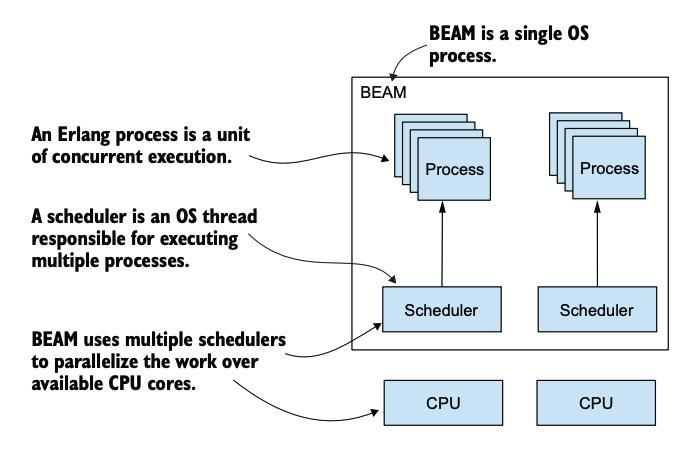
\includegraphics[width=120mm]{ch-state/assets/beam-process.png}}
    \caption[Concurrency in the Erlang virtual machine]{Concurrency in the Erlang virtual machine. Adapted from \cite{Juric2024}.}
    \label{fig:beam-process}
\end{figure}

The \gls{BEAM} scheduler is considered preemptive, meaning that assigns short execution time slices to each process. This ensures that long-running tasks do not monopolize system resources, promoting fairness and responsiveness \cite{Armstrong2013}. Also, it promotes fault tolerance characteristic by stopping processes carried with permanent faults, where on a non-preemptive scheduler could harm the overall system. Processes that are blocked due to I/O operations or waiting for messages are efficiently managed by separate threads or a kernel polling service, preventing unnecessary CPU usage and ensuring that waiting processes do not stop the execution of others \cite{Juric2024,erlang-concurrency-blog}.

\begin{figure}
    \centering
    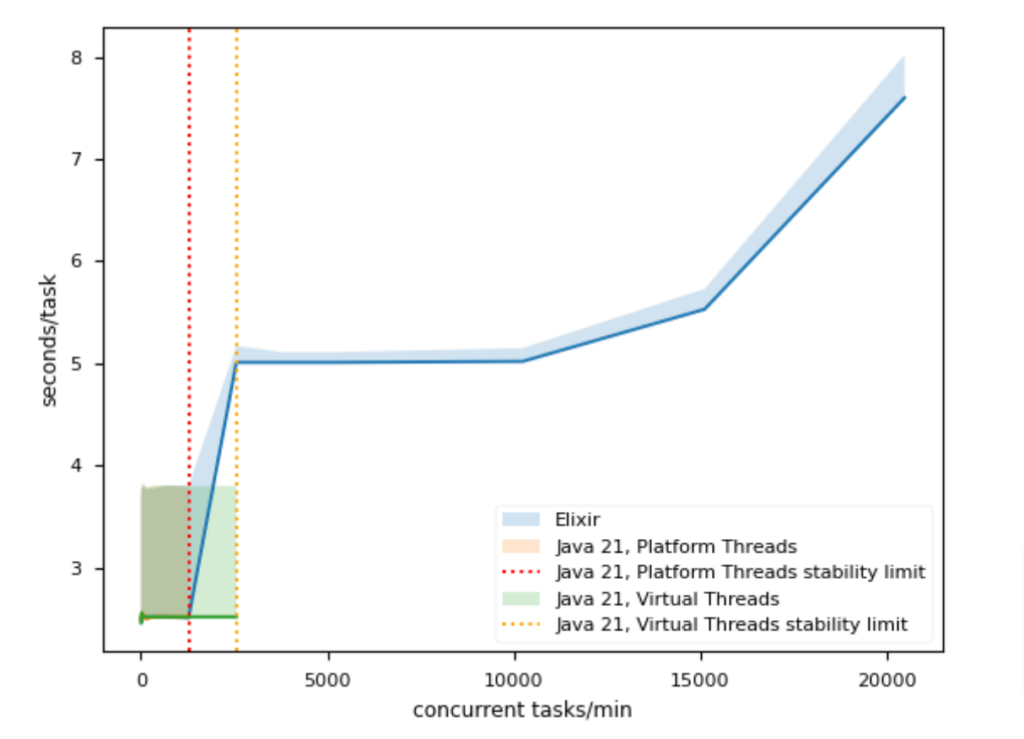
\includegraphics[width=120mm]{ch-state/assets/elixir-vs-jvm-threads.png}
    \caption[Elixir/BEAM processes vs JVM threads]{Elixir/BEAM processes vs JVM threads. Adapted from \cite{erlang-concurrency-blog}.}
    \label{fig:beam-vs-jvm}
\end{figure}

In a direct comparison of Elixir’s processes running on \gls{BEAM} with the two threading techniques of the \gls{JVM}, as illustrated in Figure \ref{fig:beam-vs-jvm}, notable differences appears. Under low load conditions, all three strategies, Elixir’s lightweight processes, the \gls{JVM}’s platform, and virtual threads, perform effectively. However, as the system approaches the stability limits of platform threads, approximately 2500 concurrent units, Elixir continues to handle additional processes, scaling up to approximately 200,000 concurrent processes. Although the per-task completion time increases slightly under such high loads, the system remains operational and stable. The opposite occurs with both \gls{JVM} techniques, resulting in an overload that makes maintaining pace impossible. Furthermore, \gls{BEAM} imposes a theoretical limit of roughly 134 millions processes, where this limit are lowered where the underlying implementation are a direct relationship with \gls{OS} threads, like what happens in \gls{JVM} \cite{Juric2024}.

This scalability advantage can be attributed to the architecture of the underlying \gls{BEAM}. Unlike the \gls{JVM}, which relies on a shared heap and tightly integrates with \gls{OS} threads. However, the \gls{JVM} threading model is better suited for low-concurrency scenarios involving long-lived threads. In contrast, Elixir/\gls{BEAM} excels in high-concurrency situations with short-lived processes \cite{erlang-concurrency-blog, Valkov2018}.

\subsubsection{Garbage Collection and Immutability}

Erlang and Elixir enforce immutability as a fundamental principle, ensuring that all data remains unchangeable. This eliminates many common concurrency issues in systems with shared memory, such as race conditions. Instead of sharing memory, processes communicate by passing immutable data. When a message is sent, the receiving process creates a copy of the data in its stack, eliminating the need for semaphore controls or similar synchronization mechanisms \cite{Juric2024,erlang-concurrency-blog}.

Because processes are completely isolated and do not share memory, \gls{BEAM} can execute garbage collection at the process level. This per-process garbage collection allows the \gls{VM} to reclaim memory for a single process without pausing the entire system, unlike the global garbage collection approach commonly used in the \gls{JVM}, where all processes share a single heap. Additionally, \gls{BEAM} optimizes garbage collection by focusing on individual schedulers enhancing its efficiency \cite{Armstrong2013,Juric2024}.

The garbage collector can significantly impact the performance of both the \gls{BEAM} and \gls{JVM}. As illustrated in Figure \ref{fig:beam-vs-jvm}, the load on \gls{BEAM} outperforms that of the \gls{JVM}. This difference may be attributed to the \gls{JVM}'s "stop-the-world" garbage collection, which can create performance bottlenecks. In contrast, \gls{BEAM} utilizes a more targeted garbage collection approach, benefiting from process isolation, which can lead to enhanced performance \cite{Valkov2018, Juric2024}.

\subsubsection{Hot-code swapping}

Hot-code swapping is a beneficial feature for building fault-tolerant systems, allowing the modification of code that is actively running in real time. This mechanism enhances fault tolerance by enabling the replacement of fault code without requiring system downtime. The process is typically achieved by sending a message to the server, which then handles the exchange \cite{Armstrong2013}.

It is important to note that this capability is not implemented in the same way on the \gls{JVM}. While the \gls{JVM} supports class reloading, it is not comparable to hot-code swapping of \gls{BEAM} and introduces significant complexities, such as managing already instantiated objects. In contrast, the hot-code swapping mechanism in systems that rely on \gls{BEAM} allow targeted changes, focused on specific parts without disrupting the system \cite{erlang-concurrency-blog}. Furthermore, in comparison with the Go language, which is a compiled language, does not permit hot code swapping in a production environment natively \cite{go-docs}.

\subsection{Fault Tolerance Mechanism and Strategies}

Elixir's fault tolerance strategies and mechanisms are associated to the Erlang ecosystem, leveraging the features of the \gls{BEAM}. A fundamental aspect of Elixir's fault tolerance is its adherence to the "let it crash" philosophy, which, combined with the actor model and extensive support from third-party tools, enhances its resilience. This is elaborated upon in the following sections.

\subsubsection{Let It Crash Philosophy and Actor Model}

Elixir inherits the “let it crash” philosophy from Erlang, which forms the foundation of its fault tolerance strategy. This philosophy is based on the principle that failures are unavoidable in distributed systems, and the optimal approach is not to prevent them entirely but to design systems that can recover autonomously and gracefully \cite{Armstrong2013, Kleppmann2017}. Instead of defensive programming to anticipate every potential error, Elixir encourages developers to isolate processes so that faults can occur without compromise the stability of the entire system \cite{Juric2024}.

The Actor Model plays a central role in achieving this resilience. In Elixir, lightweight processes act as independent actors that do not share memory and communicate exclusively through message-passing. When a process encounters an unrecoverable error, it is allowed to fail and terminate. This termination is both deliberate and beneficial, as it enables easy fault detection and ensures that failures do not propagate, preserving the integrity of the overall system \cite{Juric2024,Armstrong2013}. This model naturally integrates with the Supervisor pattern, which is one of Elixir’s primary mechanisms for fault recovery.

\textit{\underline{Supervisor Pattern}}

The Supervisor pattern is a practical implementation of the “let it crash” philosophy, built on the Actor Model. While the concept is not exclusive to Elixir, other frameworks like Akka also use it. Elixir leverage this pattern to build fault-tolerant systems \cite{Valkov2018}. In this approach, processes are classified into two types \cite{Juric2024}:

\begin{itemize}
    \item \textbf{Workers:} Processes that perform tasks or contain application logic but do not oversee other processes.
    \item \textbf{Supervisors:} Processes responsible for monitoring and managing other processes.
\end{itemize}

\begin{figure}
    \centering
    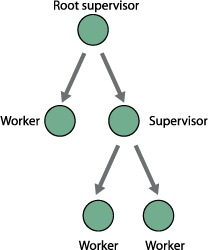
\includegraphics[scale=0.7]{ch-state/assets/supervisor-design.jpg}
    \caption[Supervisor tree pattern]{Supervisor tree pattern. Adapted from \cite{Juric2024}.}
    \label{fig:supervisor-pattern}
\end{figure}

Supervisors are organized into a hierarchical supervision tree, as illustrated in Figure \ref{fig:supervisor-pattern}. This tree defines the relationships between supervisors and workers, with each supervisor managing a group of processes. This structure provides modularity and ensures that fault recovery is localized, reducing the impact of failures \cite{Armstrong2013}.

Supervisors in Elixir operate using restart strategies to determine how to handle failures. The options given by the \gls{OTP} Supervisors, and the most common ones, are the following \cite{elixir-docs-hexdocs,Juric2024,Armstrong2013}:
\begin{itemize}
    \item \textbf{One-for-One:} If a single worker process fails, the supervisor restarts only that process.
    \item \textbf{One-for-All:} If one process fails, the supervisor restarts all processes it manages.
    \item \textbf{Rest-for-One:} If a process fails, the supervisor restarts it and all other processes started after it in the hierarchy.
\end{itemize}

Each restart strategy addresses specific use cases. Additionally, supervisors can enforce restrictions on the restart process through a restart frequency configuration. This mechanism monitors the frequency of the worker process failures within a specified time frame. If a worker process fails repeatedly and exceeds the configured threshold, the supervisor itself terminates to avoid harming the system or entering an infinite restart loop \cite{Armstrong2013}.

The One-for-One strategy is best suited for independent processes \cite{Armstrong2013}. For instance, in a web server handling multiple concurrent requests, this strategy could allow for the rapid recovery of a single failed process without affecting others. In contrast, the One-for-All strategy is ideal for tightly coupled processes \cite{Armstrong2013}. When one process fails, all other processes under the same supervisor are restarted, this could be useful for processes that need synchronization among them. Finally, the Rest-for-One strategy could be used in workflows with sequential dependencies \cite{elixir-docs-hexdocs}. For example, in a data pipeline where each stage relies on the output of the previous stage, a failure in one process triggers the restart of the failed process along with any subsequent ones.

The supervision pattern is not uniquely associated with Elixir, it is also used in other languages that follow the Actor Model, as well as in various frameworks that implement this programming style. One of the most notable \gls{JVM} frameworks is Akka. Additionally, in other paradigms such as Go, there are libraries capable of unifying \gls{CSP} with the Actor Model, such as the \textit{proto.actor} library.


\subsubsection{Tools and Support}

Elixir’s state of art in the fault tolerance area is related to the integration with the Erlang ecosystem, the \gls{BEAM}, the Actor Model, and the “let it crash” philosophy. These elements are further enhanced by Elixir’s compatibility with the \gls{OTP}, which provides a suite of design principles and tools for building fault-tolerant and distributed systems. This integration allows Elixir inherit and extend the mechanisms that have been tested and proven in real case scenarios \cite{Juric2024,Armstrong2013}.

The \gls{OTP} framework enables Elixir to use the Supervision Tree pattern, an important element on fault tolerance like described early. By combining the Supervision Tree with tools like GenServer, Elixir simplifies the management of stateful processes, facilitates concurrent operations, and ensures the efficient handling of asynchronous message passing \cite{elixir-docs-hexdocs}.

Additionally, \gls{OTP} supports features like hot-code swapping, enabling systems to update running code in real-time without downtime. The inclusion of the Mnesia distributed database within \gls{OTP} further strengthens Elixir’s fault tolerance capabilities. Mnesia allows state storage across distributed nodes, ensuring data consistency and availability even in the presence of node failures \cite{elixir-docs-hexdocs,elixir-school}.

Beyond the core features of \gls{OTP}, Elixir also includes Mix, a build tool that simplifies dependency management, testing, project configuration, and documentation generation. Mix integrates into the Elixir ecosystem, simplifying development workflows and contributing to the reliability of applications by ensuring consistent builds\cite{elixir-docs-hexdocs,elixir-school}.

In addition to the built-in capabilities of \gls{OTP}, Elixir’s ecosystem benefits from third-party projects that extend its fault-tolerant capabilities. For instance, Graft, developed by Le Brun et al. \cite{LeBrun2021} in 2019, and Ra, developed by the RabbitMq team
\footnote{Ra: \url{https://github.com/rabbitmq/ra/} (accessed 4 December 2024)}
, provide an implementation of the Raft consensus algorithm. Similarly, the Fuse library
\footnote{Fuse: \url{https://github.com/jlouis/fuse/} (accessed 4 December 2024)},
a widely-used implementation of the Circuit Breaker pattern, developed in Erlang, is also compatible with Elixir.

Another aspect of Elixir that is important to reference is its metaprogramming capabilities through macros, which allow developers to write code that generates code. This enables the Elixir codebase to be partially constructed using its own macros, extending the language's functionality and reducing boilerplate \cite{Juric2024}.

Lastly, it's important to mention the Elixir environment, which includes frameworks that enhance software development. Phoenix
\footnote{Phoenix: \url{https://phoenixframework.org/} (accessed 4 December 2024)}
is a popular framework for building scalable web applications. It inherits Elixir's fault tolerance, allowing applications to handle errors gracefully and maintain uptime. Phoenix also supports real-time features through channels for live updates \cite{Juric2024}. Nerves
\footnote{Nerves: \url{https://nerves-project.org/} (accessed 4 December 2024)}
focuses on embedded systems, leveraging Elixir's fault tolerance to create resilient IoT devices. It simplifies firmware development and management, ensuring efficient hardware and system updates while addressing fault tolerance concerns.

These integrations, extensions  demonstrate Elixir’s ability to not only leverage the proven robustness of \gls{OTP} but also adapt and grow through innovative tools and libraries, solidifying its position as a leading choice for building fault-tolerant, distributed applications.

\subsection{Drawbacks and Real Applications}

The benefits of Elixir are closely tied to the powerful features of the \gls{BEAM}, as mentioned earlier. However, there are some drawbacks to consider. One major limitation is the lack of third-party libraries, despite \gls{OTP} providing good support. Currently, it is challenging for Elixir to compete with more popular languages in this regard. Additionally, although the \gls{BEAM} has a distributed nature, its single-threaded architecture with a garbage collector makes it less suitable for fault-tolerant applications in critical systems that require fault tolerance at low level \cite{Juric2024}.Another potential drawback of Elixir is that it is a dynamically-typed programming language, which can result in errors from type mismatches or programming mistakes \cite{Cassola2020}. In contrast, languages such as Scala, Java, and Go offer advantages in this regard due to their static typing. However, there have been efforts to introduce a type system to Elixir without sacrificing the language's inherent dynamism, as demonstrated in the work of Cassola et al. \cite{Cassola2020}.

Despite these limitations, Elixir has been successfully utilized in numerous prominent projects. Taking as reference the official website of Elixir, for example, Discord relies on Elixir as the backbone of its chat infrastructure, leveraging its ability to handle real-time communication effectively. PepsiCo also employs Elixir in a central role within its data pipeline, providing marketing and sales teams with tools to query, analyze, and integrate data from various search marketing partners. Other notable examples of Elixir's application include Heroku, SparkMeter, and several others.

\section{Scala Programming Language with Akka Toolkit Analysis}

The success of the actor model, particularly through its implementation in Erlang inspired other programming languages to replicate its concepts \cite{Juric2024,Abraham2023}. Among these were languages running on the \gls{JVM}, such as Scala and Java. However, significant differences emerged due to the JVM’s inherent concurrency challenges. Unlike \gls{BEAM}, which was built with lightweight process isolation and message passing at its core, the \gls{JVM} relied on low-level thread management and shared memory, necessitating careful synchronization through locks and other mechanisms. Although this languages offered \gls{API}s for concurrency management, these general-purpose languages placed much of the responsibility on the developer \cite{Abraham2023,akka-docs}, going against the philosophy of Erlang/Elixir, that it was created for concurrency programming.

This gap on the \gls{JVM} led to the creation of the Akka toolkit, designed to bring the actor programming model to its ecosystem. Inspired by Erlang, Akka offers a runtime and comprehensive tools to support actor-based programming, enabling developers to leverage the \gls{JVM} while benefiting from a more structured approach to concurrency \cite{akka-docs}. By abstracting thread management and providing a framework for asynchronous communication and fault tolerance, Akka creates a solution to implement scalable and distributed systems \cite{Abraham2023}.

\subsection{How Akka Handles the Actor Model}

This section explores one of the two key characteristics of the actor model and how the Akka toolkit addresses it. Specifically, it describes the distributed nature and communication aspects, as well as the isolation provided by Akka. This toolkit functions as an abstraction layer built on top of Scala and the \gls{JVM}.

\subsubsection{Location Transparency and Communication}

The Actor Model, like described before, defines a concurrent paradigm where actors operate independently, maintain their own mailboxes, and communicate exclusively via message passing. This communication should ideally respect the location transparent characteristic of distributed systems, allowing actors to interact seamlessly regardless of their physical location \cite{Armstrong2013}. On the JVM, threading enables scaling within a single machine by utilizing additional CPUs and memory due to the shared heap memory and concurrency model \cite{Abraham2023}. However, native support for scaling across distributed systems is lacking, a contrast to BEAM’s distributed aspect.

BEAM facilitates seamless inter-process communication natively, as previously discussed. Akka addresses this limitation through its latest remoting protocol, Artery, which builds upon the older remoting mechanisms making improvements \cite{akka-docs,Abraham2023}. Artery employs either TCP or Aeron UDP for communication. While Aeron UDP delivers high throughput and low latency, it lacks encryption, making it suitable for specific trusted environments. TCP, on the other hand, offers encrypted communication with similarly high throughput, although with potentially higher latency under extreme load \cite{akka-docs}. Unlike BEAM’s native capabilities, Akka’s abstractions inevitably introduce some overhead to the communication between actors.

Akka facilitates scalability and communication with the discovery module. The discovery module serves a purpose similar to namespaces in Elixir, allowing actors to be registered with a specific name. In this context, actors can be registered using a designated key \cite{Abraham2023}, and other actor can communicate with that name without knowing the specific address. Furthermore, communication with these actors occurs through their mailboxes, following a standard First-In-First-Out (FIFO) protocol, equals to the behavior in Elixir \cite{Moamen2027,Juric2024}.

\subsubsection{Actors Isolation}

Actor isolation is a foundational principle of the Actor Model, where actors are designed to operate independently and avoid shared state \cite{Armstrong2013}. In Java, this independence can be implemented using low-level concurrency mechanisms, while in Scala it is often achieved through immutability. However, Akka significantly simplifies the process by providing an Actor API that inherently enforces isolation \cite{Abraham2023,Bagherzadeh2020}. Initially, Akka introduced the Classic Actors API, which supported untyped actor logic. In this model, messages were transmitted without type safety and processed using pattern matching, similar to the approach employed in Elixir \cite{akka-docs}. In contrast, the modern standard is the Typed Actor API, which provides a more robust and type-safe solution. The Typed Actor API enforces type safety through, ensuring that only messages of the defined type can be sent to an actor \cite{Abraham2023,akka-docs}. This differs from Elixir, where actor communication is dynamically typed and does not provide type guarantees.

Unlike Elixir, Scala permits mutable programming, which introduces the potential for shared mutable data to be passed between actors, a practice strongly discouraged in Akka’s documentation. Despite these guidelines, the use of mutable data within Akka is technically possible. If misused, this could reintroduce well-known concurrency issues in the JVM, such as race conditions and thread interference \cite{akka-docs}. This limitation stands in contrast to Elixir’s approach, where the \gls{VM} guarantees strict process isolation, effectively eliminating such risks \cite{Juric2024,Valkov2018}.

To achieve efficient performance, actors in Akka often share underlying threads, as individual threads are resource-intensive \cite{Moamen2027}. Akka actors mimic the lightweight processes of the \gls{BEAM} by managing multiple actors within a single thread. This approach significantly reduces memory consumption compared to the heavyweight \gls{JVM} threads. For instance, approximately 2.7 million Akka actors can fit within 1 GB of memory, a considerable contrast to the 4,096 threads that would occupy the same space \cite{Abraham2023}

\begin{comment}

\textit{\underline{Messager Dispatchers}}

Message dispatchers plays a important role in Akka’s architecture by managing the execution of actor tasks. A dispatcher serves as the mechanism that determines how messages are delivered to actors and how these actors are allocated to threads for execution. The default dispatcher is a thread pool executor based on the Fork/Join framework, enabling high concurrency with minimal overhead.

The flexibility of Akka dispatchers allows for fine-grained control over thread allocation, ensuring efficient utilization of system resources. For example, the pinned dispatcher assigns each actor its own dedicated thread, suitable for actors requiring uninterrupted execution. Conversely, the default dispatcher facilitates efficient thread sharing across a large number of actors. This configurability enables developers to tailor Akka’s performance characteristics to their application’s specific needs, such as minimizing latency or maximizing throughput.

Elixir’s message dispatching model, in contrast, is built into the \gls{BEAM} and abstracts much of the configuration from the developer. While this simplicity is advantageous, it lacks the level of customization offered by Akka. However, the \gls{BEAM}’s design provides guarantees of fairness and isolation, attributes that are less rigidly enforced in JVM-based systems, where developers must explicitly manage such concerns.

\textit{\underline{Garbage Collector}}

Another significant topic is garbage collection. As mentioned earlier, the \gls{BEAM} focuses on localized updates within individual processes, which allows for process-specific garbage collection. This ensures minimal disruption, as garbage collection can occur independently across processes. In contrast, the JVM employs heap-based garbage collection, which can trigger global stop-the-world pauses. Despite of  These pauses introduce the risk of application latency spikes or even node failures under high load. This fundamental difference highlights a critical limitation of JVM-based actor systems like Akka compared to the \gls{BEAM}, where garbage collection aligns more naturally with the principles of actor isolation.
\end{comment}

\subsection{Fault Tolerance Mechanism and Strategies}

Akka, built upon the Actor Model, inherits its fault-tolerance philosophy from Erlang’s design principles, like described on Elixir's section. This is the foundation of the fault tolerance aspects, at its core, the Actor Model facilitates fault tolerance through the supervisor pattern. By defining strategies for handling failures, such as restarting, stopping, or resuming child actors, supervisors ensure that errors are contained and localized, preventing system-wide failures \cite{akka-docs,Abraham2023,Juric2024}, like it was detailed before.

In addition to its foundational fault-tolerance mechanisms, Akka’s modular environment offers some modules that extend the toolkit’s capabilities, many of which directly contribute to improving fault tolerance.

\subsubsection{Akka Clustering}

Akka Cluster is a module that enables peer-to-peer communication among a group of nodes, allowing them to function as a unified distributed system \cite{Moradi2023,akka-docs}. Designed to enhance fault tolerance, it implements replication and redundancy strategies while achieving location transparency through the Artery protocol, enabling nodes to communicate without knowing the physical locations of others \cite{Abraham2023}.

The module provides an API for managing cluster operations, including managing nodes, designating a leader node, and obtaining cluster information. Although, Akka Cluster is autonomous, capable of redistributing workloads and managing actor states without manual intervention via API \cite{Abraham2023}. To ensure consistency and reliability, Akka Cluster employs a gossip protocol, a decentralized communication mechanism that facilitates the propagation of information across nodes \cite{Tanenbaum2023,akka-docs}. This protocol enables nodes to maintain a shared, consistent view of the cluster state \cite{Tanenbaum2023}.

For job processing, Akka Cluster employs a divide-and-conquer architecture through the use of master and worker actors. The master actor decomposes large tasks into smaller subtasks, distributing these among worker actors for parallel processing. Once processing is complete, the workers return their results to the master actor, which aggregates them to produce the final output. This design enhances performance and fault tolerance, as the master actor can reassign tasks from failed workers to other available nodes \cite{akka-docs}.

Leader election is a important aspect of a cluster management, and it is efficiently managed within Akka Cluster. In contrast to the Raft consensus, algorithm Akka Cluster adopts a simpler method by automatically assigning the leadership role to the node with the lowest address. This approach minimizes the overhead associated with the election process \cite{raft-diego,akka-docs}.

Furthermore, Akka Cluster supports advanced features such as cluster sharding, which distributes actors across the cluster while preserving their identity and state. This facilitates load balancing and enhances performance by ensuring that workloads are distributed evenly. The module also includes monitoring and health management capabilities, enabling to verify the performance and status of nodes and actors \cite{Abraham2023}.

\subsubsection{Akka Circuit Breaker}

Akka provides a dedicated module for implementing the Circuit Breaker pattern, a technique for improve system stability by isolating faults and preventing cascading failures. As presented earlier, the Circuit Breaker pattern temporarily suspends operations to a failing component, allowing it time to recover while safeguarding the overall system \cite{fowler-circuit-breakers}.

Akka’s Circuit Breaker module offers a straightforward integration, making it possible to configure the way the circuit it will activate, where it can be defined failure thresholds, timeouts, and recovery intervals. This module is effective in monitoring interactions between actors and external services, ensuring that errors are contained and managed without disrupting the broader system \cite{akka-docs}.

Compared to Elixir’s ecosystem, where circuit breaker functionality often relies on third-party libraries, Akka’s Circuit Breaker benefits from being a native part of its comprehensive toolkit.

\subsubsection{Akka Persistence and Event Sourcing}

Akka also provides support for fault tolerance through mechanisms such as message logging and check-pointing. Akka Persistence with event sourcing enables actors to recover their state following a failure, ensuring consistency in system behavior. This is achieved by maintaining an event log that records all changes to an actor’s state in the order they occurred. Upon a restart, often triggered by a supervisor, the actor replays the logged events to reconstruct its previous state, effectively resuming operations from where it left off before the crash \cite{akka-docs}.

To optimize the recovery process, Akka Persistence also supports snapshots, supporting also the check-pointing strategy. Instead of replaying all events from the beginning of the event log, the actor can restore its state from the most recent snapshot and then replay only the events that occurred after that snapshot \cite{Abraham2023,akka-docs}.

\subsection{Comparison with Elixir/BEAM and Real Applications}

The Akka toolkit represents a significant advancement in extending the \gls{JVM} to support modern concurrency models. As noted by Valkov et al. \cite{Valkov2018}, Akka enhances Scala’s performance by reducing communication latency, making it a powerful tool for building reactive systems. However, it operates as an abstraction layer on top of the \gls{JVM}, while the \gls{BEAM} virtual machine is inherently designed as a state of the art concurrency platform \cite{erlang-concurrency-blog}. The \gls{JVM} was originally created to address general-purpose programming needs with a focus on efficiency, but it does not inherently prioritize the actor model or process-level isolation as the \gls{BEAM} does.

\textbf{Garbage Collection.} A notable difference between Akka and the \gls{BEAM} lies in their approach to garbage collection. Akka relies on the \gls{JVM}’s garbage collection strategy, which can introduce latency during stop-the-world events \cite{akka-docs,Abraham2023}. These pauses can negatively affect the performance of highly concurrent systems, especially under heavy load. However, advancements in garbage collection technology, such as the Z Garbage Collector, have shown possibilities in reducing pause times significantly. As noted by Chaudhary et al. \cite{Chaudhary2024}, Z Garbage Collector represents a state of the art approach that is well-suited for applications requiring minimal pauses due to garbage collection. In contrast, the \gls{BEAM} employs a per-process garbage collection mechanism, which localizes memory management to individual lightweight processes \cite{Juric2024}. This architecture ensures that garbage collection in one process does not impact others, making the \gls{BEAM} particularly effective in low-latency and high-reliability scenarios.

\textbf{Scheduling Model.} Scheduling represents a fundamental difference between Akka and the \gls{BEAM}. The \gls{BEAM} employs a preemptive scheduling model designed to efficiently handle numerous small, short-lived tasks, such as high-frequency message handling in highly concurrent systems. This approach ensures equitable CPU time distribution and mitigates process starvation \cite{Juric2024,elixir-docs-hexdocs,erlang-concurrency-blog}. However, frequent context switching can introduce overhead for long-running processes, potentially reducing efficiency in such scenarios. Akka, on the other hand, relies on the \gls{JVM}’s cooperative scheduling model and enhances it with its Message Dispatcher, which supports configurable thread pools like Fork-Join, that leverages a work-stealing algorithm, and Fixed Thread Pools, optimizing resource usage. This mechanism enables Akka to efficiently manage long-lived and computationally intensive tasks \cite{akka-docs,Abraham2023}.

\textbf{Built-in Libraries and Support.} Both the Akka and Elixir/\gls{BEAM} ecosystems offer comprehensive libraries to address common design patterns for concurrency and fault tolerance. Elixir’s \gls{OTP} framework, like stated before, provides a robust suite of built-in patterns, such as supervisors, specifically tailored for managing concurrency and ensuring system reliability \cite{erlang-concurrency-blog,elixir-docs-hexdocs}. Akka, on the other hand, adopts a modular architecture with an easily pluggable library of features, including implementations for replication and circuit breakers. In the Elixir ecosystem, equivalent functionality is often achieved through third-party libraries maintained by the community. While these community-driven libraries are highly effective and widely used, their reliance on external maintenance and updates can present a potential drawback compared to Akka’s more integrated and officially supported approach.

\textbf{Real-World Applications.} Akka, just as Elixir, has demonstrated its capabilities in considerable large-scale applications, emphasizing its scalability, reliability, and performance. For instance, PayPal leverages Akka actors to manage over a billion financial transactions daily, ensuring high availability and robust fault tolerance \cite{Bagherzadeh2020}. Similarly, the Spark big data ecosystem depends on Akka for efficiently shuffling hundreds of terabytes of data across distributed nodes. Other prominent companies, including Twitter, LinkedIn, and Walmart use Akka to solve concurrency and distributed system challenges \cite{Bagherzadeh2020,akka-docs}.

\section{Go Programming Language Analysis}

The Go programming language was designed to facilitate rapid software development while ensuring high execution speed \cite{Kennedy2016, Cox-Buday2017}. It addresses the drawbacks of traditional low-level languages like C, which, while performant, can be complex for modern development. At the same time, Go offers a solution to the performance limitations of scripting languages such as Python, which prioritize ease of use but often fails in execution speed \cite{Kennedy2016}. As a statically typed, compiled language, Go enforces type safety \cite{go-docs}, setting it apart from dynamic and immutable languages like Elixir, as well as frameworks like Akka that also emphasize immutability.

While Go is not explicitly classified as a distributed or fault-tolerant programming language, it has gained considerable popularity in areas such as microservices, cloud applications, and high-concurrency systems. This popularity can be attributed to its simplicity, speed, and robust concurrency model \cite{Castro2019,Shuiskov2022}. In contrast to Elixir, which is designed with immutability and a let it crash fault-tolerance philosophy, Go does not inherently prioritize fault tolerance or the let it crash approach \cite{Cox-Buday2017}. Nevertheless, Go can be a good candidate for integration into distributed architectures when paired with complementary technologies. By take advantage of Go’s concurrency capabilities, it is possible to replicate certain fault-tolerant strategies typical of Elixir-based systems, making it a valuable language to explore in this context.

\subsection{Concurrency and Distribution in Go}

Go adopts a concurrency model rooted in the \gls{CSP} paradigm, distinguishing itself from other approaches such as the Actor Model. While both paradigms prioritize concurrent communication, they are slightly different in their focus \cite{Cox-Buday2017}. In \gls{CSP}, channels are treated as first-class entities, emphasizing the communication mechanism itself, whereas the Actor Model considers processes to be first-class, focusing on the entities performing the computation, as described earlier. Additionally, the Actor Model enforces strict isolation between processes, with no shared memory, while CSP organizes concurrent processes to interact explicitly through channels rather than directly access to a single shared memory object \cite{Cox-Buday2017}. 

Go is one of the first programming languages to integrate \gls{CSP} directly into its design, emphasizing data sharing through channels rather than passing references to shared memory among its lightweight threads, known as goroutines \cite{Cox-Buday2017}. This design choice minimizes potential synchronization complexities and aligns with Go’s guiding principle: “Do not communicate by sharing memory; instead, share memory by communicating” \cite{go-docs}. This philosophy contrasts with shared-memory concurrency models, where processes directly access and modify shared state. In Go, by design, only one goroutine can access a value at any given time, effectively eliminating the possibility of data races \cite{Kennedy2016,go-docs}. Nevertheless, Go also provides manual synchronization mechanisms, such as explicit mutexes, for situations where they are necessary \cite{Cox-Buday2017}.

In contrast to the Actor Model, where actors encapsulate state and communicate through asynchronous messages, Go’s \gls{CSP}-based model prioritizes structured communication patterns via channels. This distinction encourages developers to design systems by focusing on the flow of data and the relationships between processes, rather than the individual behavior of the computational units \cite{go-docs}.

Go's strategy utilizing \gls{CSP} is centered around goroutines and channels, which are described below. Additionally, it will be briefly discuss how Go's garbage collector operates, as well as the limitations of channels and goroutines in supporting distributed communication.

\subsubsection{Goroutines}

Due to the overhead associated with \gls{OS} threads, Go enhances efficiency by implementing a multiplexing logic that allows multiple processes to run on the same \gls{OS} thread \cite{Cox-Buday2017,Castro2019}, similar to the approaches used in Elixir and Akka. Go achieves this through goroutines, which are lightweight abstractions that enable concurrent and parallel execution. By utilizing goroutines, Go can efficiently manage numerous tasks without significant resource consumption \cite{go-docs}.

The \gls{OS} is responsible for scheduling threads to run on physical processors, whereas Go handles the scheduling of lightweight goroutines onto logical processors, which are subsequently bound to \gls{OS} threads \cite{Kennedy2016}. As shown in Figure \ref{fig:gorutine-threads-relation}, the example illustrate two \gls{OS} threads (M2 and M3), with goroutines identified by the prefix \textit{G}. The scheduling process involves allocating goroutines to logical processors via a local run queue. However, initially, goroutines are placed in the global scheduler run queue, and only afterward are they assigned to the local queues of logical processors \cite{Kennedy2016,Cox-Buday2017}. The same Figure \ref{fig:gorutine-threads-relation}, also illustrates how Go achieves parallelism. Goroutines can be distributed across multiple CPU cores if the hardware supports parallel execution \cite{Kennedy2016}.

\begin{figure}
    \centering
    \frame{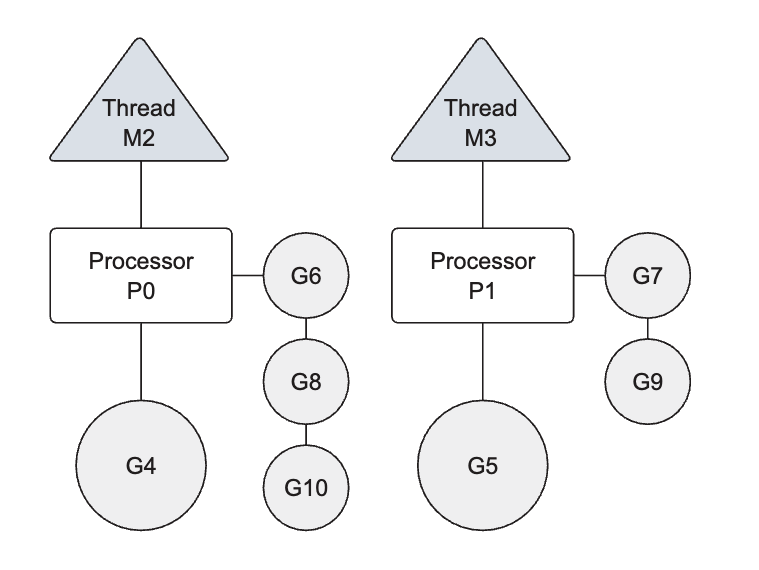
\includegraphics[width=100mm]{ch-state/assets/goroutine-threads-relation.png}}
    \caption[Go’s scheduler logic of distributing goroutine by the logical processors]{Go’s scheduler logic of distributing goroutine by the logical processors. Adapted from \cite{Kennedy2016}.}
    \label{fig:gorutine-threads-relation}
\end{figure}

\subsubsection{Channels}

Building on the \gls{CSP} model, Go integrates channels as a core element of its concurrency paradigm. These data structures facilitate safe and efficient communication between goroutines, enhancing synchronization while addressing common challenges associated with shared memory access \cite{Kennedy2016}. By following the principle that only one goroutine should modify a piece of data at any given time, channels help ensure data integrity, reducing the risk of concurrent modification and giving predictable behavior in concurrent programs \cite{Cox-Buday2017}.

However, channels in Go do not inherently enforce data access protection features such as immutability and isolation \cite{Kennedy2016}, which are fundamental to the concurrency models found in languages like Elixir and Scala with Akka. These languages are specifically designed to facilitate effective concurrency management, like analyzed earlier. Nevertheless, it is possible to adopt a strategy of using immutable data within Go channels, where all information is a copy of the original data \cite{Cox-Buday2017}. This approach aligns more closely with the methodologies employed by Elixir and Scala, even though it is not the primary purpose of channels in Go.

\subsubsection{Garbage Collector}

In Go, the garbage collection strategy is based on a concurrent, non-generational mark-and-sweep algorithm \cite{go-docs}, which operates globally on the heap \cite{Zhao2023}. This approach differs significantly from the BEAM VM's garbage collector, which performs garbage collection on a per-process basis. The BEAM VM’s process-level garbage collection minimizes the impact on overall system performance by isolating garbage collection events to individual processes \cite{Juric2024}.

Go's garbage collector, while global in nature, supports partial heap collection but still experiences "stop-the-world" pauses. Despite these challenges, it is designed to maintain pause times between 10 ms and 100 ms under heavy load, making it comparable to the G1 garbage collector in the JVM, which, as studied by Zhang et al. \cite{Zhang2021}, can experience pause times ranging from 0 to 300 ms. In contrast, ZGC achieves significantly lower pause times, typically between 0 and 0.1 ms, making it an attractive option for latency-sensitive applications, although it is not compatible with Go's environment \cite{Castro2019}.

Each garbage collection approach has its own advantages and trade-offs. Elixir’s garbage collection, rooted in the BEAM runtime, is particularly well-suited for distributed programming due to its strong emphasis on process isolation \cite{Armstrong2013}. In contrast, Go supports a partial heap-targeted garbage collector, which pairs effectively with its lightweight goroutines, enhancing memory management in concurrent applications.

\subsubsection{Distributed Communication}

A notable limitation of Go is its lack of native support for distributed communication \cite{Whitney2019, Cox-Buday2017}. While the combination of channels and goroutines serves as an excellent tool for managing concurrency and parallelism, it does not inherently extend to communication across physical machines \cite{Kennedy2016}. This limitation has prompted efforts to extend Go’s concurrency model to support distributed systems. For instance, Whitney et al. \cite{Whitney2019} proposed a novel protocol called Gluster, which provides a library to abstract cluster logic and facilitate distributed communication. However, Gluster has seen limited industrial adoption and is restricted to Linux environments, limiting its general applicability.

Nevertheless, Go it offers seamless integration with mature and optimized networking libraries \cite{Kennedy2016}. Packages such as \gls{TCP}, \gls{HTTP}, and \gls{gRPC} provide efficient mechanisms for enabling communication between distributed components \cite{Castro2019, go-docs}. These libraries significantly reduce the overhead associated with managing low-level networking concerns. Furthermore, channel-based networking libraries allow the management of distributed interactions effectively, leveraging goroutines and channels to handle the inherent asynchronous aspects of the network calls \cite{Castro2019}.

While Go’s native concurrency primitives do not align with the Actor Model, there are projects of the Actor Model available for the Go ecosystem. One mature example is Proto-Actor \cite{Whitney2019,proto-actor-docs}, a library that abstracts the complexities of distribution through its \gls{API}. Built on top of \gls{gRPC}, Proto-Actor provides a remote facilities and location transparency of the Actor Model within Go \cite{proto-actor-docs}.

Go’s rising popularity in the industry is closely tied to its adoption in microservices architectures and cloud-native applications \cite{Zhao2023,Shuiskov2022}. Microservices, by their nature, represent distributed systems and facilitate communication through both asynchronous and synchronous methods, often utilizing discovery services to map all nodes. Another approach involves the use of message queues, which can provide location transparency for processes \cite{Shuiskov2022}. However, these strategies may lead to over-engineering, in some cases, resulting in additional overhead compared to the native approach of Elixir.

\subsection{Fault Tolerance Mechanism and Strategies}

Go's approach to fault tolerance is not a central feature of the language, particularly in contrast to Elixir's "let it crash" philosophy. Instead, Go has a more explicit error-handling strategy that emphasizes direct management of errors. Also, to achieve fault-tolerance capabilities similar to those of Elixir and Akka, it is often necessary to rely on specific patterns and libraries.

\subsubsection{Error Philosophy}

Until now, the “Let it crash” philosophy has been described, a core principle applied in both Elixir and Akka due to the inherent design of the Actor Model. This approach is based on the inevitability appearance of errors, allowing them to occur and relying on mechanisms like the supervisor pattern to detect and recover from them \cite{Armstrong2013}. However, the error-handling philosophy in Go is fundamentally different, representing almost the opposite paradigm. In Go, the strategy emphasizes handling every error explicitly \cite{Kennedy2016,go-docs}. Errors are treated as first-class citizens, returned as values, and must be actively managed by the program. Unlike languages such as Java and even Elixir \cite{elixir-docs-hexdocs}, Go does not include mechanisms like try-catch for error handling. Instead, it enforces a more explicit style that requires developers to check for and respond to errors immediately after an operation \cite{Cox-Buday2017}.

This philosophy aligns with Go’s overall design principles of simplicity, clarity, and explicitness. By requiring developers to handle errors explicitly, Go minimizes the risk of overlooking potential issues. While this approach can result in more verbose code, it aims to reduce the likelihood of unhandled exceptions and promote a clearer method of error management \cite{Kennedy2016, go-docs}.

Another important consideration in Go’s error handling philosophy is its impact on code readability and maintainability. The explicit nature of error handling in Go often leads to repetitive code blocks, resulting in more boilerplate compared to the code styles of Elixir and Akka \cite{Kennedy2016, go-docs}. However, this explicitness can facilitate tracing how errors are propagated and resolved within a program. In distributed systems, this approach can complement techniques such as logging and monitoring, contributing to overall system robustness.

\subsubsection{Fault Tolerance Mechanisms and Strategies}

While Go was not primarily designed with built-in fault tolerance mechanisms, as it emphasizes efficiency and simplicity, it has become a fundamental component in distributed systems, such as Kubernetes \cite{Castro2019, Kennedy2016}. When combined with appropriate patterns, architectural approaches, and libraries, Go enables the development of fault tolerance capabilities within these systems.

A more suitable approach in Go combines the heartbeat pattern with panic/recover mechanisms \cite{Cox-Buday2017}. In this pattern, a goroutine functions as a supervisor, monitoring other goroutines through periodic status updates known as heartbeats or pulse. If a monitored goroutine fails to send a notification within the expected timeframe, the supervisor can initiate recovery procedures to restore the failed component's state \cite{Cox-Buday2017, go-docs}. This ensures that failures are detected and addressed promptly. Furthermore, the supervision mechanism can be enhanced by Go's panic/recover pattern, which enables the system to capture and handle critical errors. This approach is similar to the supervision trees in Elixir and Akka, but it operates on a more specific and internal level, rather than addressing distributed aspects \cite{go-docs}.

A notable case study for this dissertation is Go's implementation of the Actor Model \cite{Whitney2019}. Roger Johansson, the creator of Akka.NET, with his team created an innovative approach to implementing the Actor Model in Go. This implementation demonstrates that the Actor Model can be effectively combined with \gls{CSP}, as these paradigms are complementary rather than mutually exclusive \cite{proto-actor-docs}. Proto-Actor, positioned as a next-generation Actor Model framework, introduces the "Actor Standard Protocol," which establishes a language-agnostic protocol for communication across different programming languages \cite{proto-actor-docs}. 

This implementation incorporates the fault tolerance aspects of the "let it crash" philosophy and location transparency \cite{proto-actor-docs} within the Go language. It leverages gRPC and HTTP/2 \cite{proto-actor-docs}, employing a more recent strategy compared to Akka’s Artery protocol and Erlang protocol. While this approach capitalizes on Go's efficiency, it remains a library-based implementation similar to Scala's Akka, which introduces some overhead. However, there are two key differences in execution: Akka runs on the JVM, while Go applications compile directly to machine code, potentially leading to different performance outcomes.

%Circuit breakers represent another pattern for fault tolerance in distributed applications \cite{fowler-circuit-breakers}. This pattern, being more generic and language-agnostic, prevents cascading failures by monitoring the health of dependent services or components and temporarily disabling failing components to prevent system-wide degradation \cite{fowler-circuit-breakers,Shuiskov2022}. The pattern integrates particularly well with Go's microservices architecture \cite{Shuiskov2022}.

In the context of microservices architecture, Go provides robust support through the mature Go-kit library \cite{go-kit-docs}. This library facilitates the development of microservices and distributed systems by implementing essential patterns such as circuit breakers, rate limiters, and distributed tracing capabilities \cite{go-kit-docs, Shuiskov2022}. Additionally, this framework can be enhanced with the failsafe-go library, which introduces additional aspects of fault tolerance, such as retry policies. Furthermore, integrating HashiCorp's Raft implementation can provide strong consistency and leader election capabilities.

Many of these solutions can be viewed as generic strategies that are more architectural than native, relying on third-party libraries. This is similar to the practices observed in Elixir, which frequently utilizes third-party solutions for replication, as well as in Akka for Scala. Nevertheless, the approaches outlined are effective and can capitalize on Go's popularity and efficiency.

\subsection{Challenges Compared With Akka and Elixir and Real Applications}

After examining the Go language, it is clear that it does not lend itself to fault tolerance mechanisms as naturally as Scala with Akka or Elixir. However, similar to how Akka enhances Scala, Proto-Actor leverages the combination of CSP with the Actor Model in Go \cite{proto-actor-docs}. Just as Elixir relies on third-party libraries to implement Raft consensus, Go also requires external libraries to achieve fault tolerance capabilities. Nevertheless, it easy to observe that Elixir's environment is robust and natively implements these features, providing a distinct advantage and a more convenient approach.

\textbf{Maintainability and Readability of the Code.} One of the primary challenges when using Go for fault tolerance is the maintainability and readability of the code. While Go emphasizes simplicity and clarity, the absence of built-in fault tolerance mechanisms can lead to more complex code structures when implementing custom solutions \cite{go-docs}. In contrast, Elixir and Akka provide clear abstractions for fault tolerance, such as supervision trees and actor models, which inherently promote maintainability. 

\textbf{Built-in Libraries and Support.} While Go has a growing ecosystem of libraries that facilitate fault tolerance, such as Go-kit and Proto-Actor, it lacks the extensive built-in support that Elixir and Akka offer. Elixir's OTP provides a rich set of libraries and tools specifically designed for building fault-tolerant systems, while Akka's actor model is deeply integrated into the framework. 

\textbf{Real-World Applications.} Go is widely utilized in cloud applications and high-performance systems \cite{Zhao2023}. It plays a crucial role in platforms like Docker and Kubernetes, and it has been adopted by Dropbox, which transitioned from Python to Go to achieve greater efficiency \cite{go-docs}. Another success story is Cockroach Labs, which has noted that Go's garbage collection and performance are well-suited for their needs \cite{go-docs}. However, there are challenges as well. For instance, Discord initially attempted an implementation in Go but ultimately migrated to Rust. This decision was influenced by issues related to Go's garbage collection, which caused significant latency spikes, leading to the conclusion that the garbage collector contributed to performance degradation \cite{discord-blog-rust-go}. It is important to note that the effectiveness of garbage collection can depend on the specific use case and workload, as different applications may have varying requirements and tolerances for latency.

\section{Benchmarking Strategies}

% - https://dl.acm.org/doi/pdf/10.1145/2541329.2541339

% - mutation tests in akka: https://dl.acm.org/doi/pdf/10.1145/3611643.3616362

\section{Conclusions}